\documentclass[10pt]{article}
\usepackage[margin=0.8in]{geometry}
\usepackage[utf8]{inputenc}
\usepackage[T1]{fontenc}
\usepackage{graphicx}
\usepackage[export]{adjustbox}
\usepackage{amsmath}
\usepackage{amsfonts}
\usepackage{amssymb}
\usepackage[version=4]{mhchem}
\usepackage{stmaryrd}
\usepackage{bbold}
\usepackage{fixltx2e}
\usepackage{caption}
\usepackage{mathtools}
\usepackage[parfill]{parskip}
\usepackage{float}
\usepackage{amsmath}

\usepackage[framemethod=TikZ]{mdframed}
\colorlet{shadecolor}{orange!15}
\usepackage{xcolor}
\usepackage{amsthm}
\usepackage{framed}

\begin{document}


\title{Lecture 21: Centralized Joint Control}
\author{Wanxin Jin}
\maketitle

In the previous sections, we have discussed the design of independent joint controllers. These are based on a single input/single-output approach, and the coupling effects between
the joints have been considered as disturbances acting on each single joint. When large operational speeds are required, or direct drive actuation is used $\left(\boldsymbol{K}_{r}=\boldsymbol{I}\right)$, the nonlinear coupling terms strongly influence system performance. Thus, considering the effects of the components of $\boldsymbol{d}$ as a disturbance may generate large tracking errors. In this case, it is advisable to design control algorithms that take advantage of a detailed knowledge of manipulator dynamics to compensate for the nonlinear coupling terms of the model. This leads to centralized control algorithms.


In the following control design for a $n$-joint manipulator, we consider a manipulator without external end-effector forces  and  any joint friction.   The equation of motion of the manipulator thus is 

\begin{equation}\label{equ.manipulator}
    \boldsymbol{B}(\boldsymbol{q}) \ddot{\boldsymbol{q}}+\boldsymbol{C}(\boldsymbol{q}, \dot{\boldsymbol{q}}) \dot{\boldsymbol{q}}+\boldsymbol{g}(\boldsymbol{q})=\boldsymbol{\tau}.
\end{equation}

The controller we want to design is in the general form of 
\begin{equation}\label{equ.controller}
\boldsymbol{\tau}=\boldsymbol{u}=\textbf{Controller}(\boldsymbol{q}, \boldsymbol{\dot{q}}, \boldsymbol{q}_d, \boldsymbol{\dot{q}}_d)
\end{equation}
i.e., the controller takes as input the manipulator's current joint position $\boldsymbol{q}$, current joint velocity $\boldsymbol{\dot{q}}$, the desired joint position $\boldsymbol{q}_d$, and desired joint velocity $\boldsymbol{\dot{q}}_d$, and outputs the joint torque $\boldsymbol{u}$.

Thus, the controlled manipulator  with the controller  is 
\begin{equation}\label{equ.manipulator_control}
    \boldsymbol{B}(\boldsymbol{q}) \ddot{\boldsymbol{q}}+\boldsymbol{C}(\boldsymbol{q}, \dot{\boldsymbol{q}}) \dot{\boldsymbol{q}}+\boldsymbol{g}(\boldsymbol{q})=\textbf{Controller}(\boldsymbol{q}, \boldsymbol{\dot{q}}, \boldsymbol{q}_d, \boldsymbol{\dot{q}}_d)
\end{equation}

\section{Controller I: PD Control with Gravity Compensation}


Given a \emph{constant} desired joint position  $\boldsymbol{q}_{d}$, we want to design a controller (\ref{equ.controller}), such that  from  any initial configuration, say $\boldsymbol{q}_0$, the controlled manipulator (\ref{equ.manipulator_control}) will eventually reach $\boldsymbol{q}_{d}$. If we define the joint space error as  the error between the desired and the actual joint positions:
\begin{equation}
    {\boldsymbol{e}}=\boldsymbol{q}_{d}-\boldsymbol{q}
\end{equation}
we want 
$$
\boldsymbol{e}(t)\rightarrow \boldsymbol{0}\quad \text{as}\quad
t\rightarrow \infty.
$$

Below, we will design the controller (\ref{equ.controller}) based on the Lyapunov method (see  background of Lyapunov method in Lecture 16-17). First, we take the vector $\begin{bmatrix}\boldsymbol{e}\\
\boldsymbol{\dot{q}}\end{bmatrix}$  as the control system state. Choose the following positive definite quadratic form as Lyapunov function candidate:

$$
V(\dot{\boldsymbol{q}}, {\boldsymbol{e}})=\frac{1}{2} \dot{\boldsymbol{q}}^{T} \boldsymbol{B}(\boldsymbol{q}) \dot{\boldsymbol{q}}+\frac{1}{2} {\boldsymbol{e}}^{T} \boldsymbol{K}_{P} {\boldsymbol{e}} \quad >0 \quad \forall \dot{\boldsymbol{q}}, {\boldsymbol{e}} \neq \mathbf{0}
$$

where $\boldsymbol{K}_{P}$ is an $(n \times n)$ symmetric positive definite matrix. 
Differentiating  $V(\dot{\boldsymbol{q}}, {\boldsymbol{e}})$ with respect to time, and recalling that $\boldsymbol{q}_{d}$ is constant, yields

$$
\dot{V}=\dot{\boldsymbol{q}}^{T} \boldsymbol{B}(\boldsymbol{q}) \ddot{\boldsymbol{q}}+\frac{1}{2} \dot{\boldsymbol{q}}^{T} \dot{\boldsymbol{B}}(\boldsymbol{q}) \dot{\boldsymbol{q}}-\dot{\boldsymbol{q}}^{T} \boldsymbol{K}_{P} {\boldsymbol{e}}
$$

From (\ref{equ.manipulator}), we can solve for $\boldsymbol{B} \ddot{\boldsymbol{q}}$ and substituting it to the above equation gives


\begin{equation}
    \label{equ.lypuanovdot}
    \dot{V}=\frac{1}{2} \dot{\boldsymbol{q}}^{T}(\dot{\boldsymbol{B}}(\boldsymbol{q})-2 \boldsymbol{C}(\boldsymbol{q}, \dot{\boldsymbol{q}})) \dot{\boldsymbol{q}}+\dot{\boldsymbol{q}}^{T}\left(\boldsymbol{u}-\boldsymbol{g}(\boldsymbol{q})-\boldsymbol{K}_{P} {\boldsymbol{e}}\right)
\end{equation}


The first term on the right-hand side is zero since the matrix $\boldsymbol{N}=\dot{\boldsymbol{B}}-2 \boldsymbol{C}$ is a skew-symmetric matrix (see in the property of dynamics in Lecture 18). For the second term to be  negative definite, we can take the controller (\ref{equ.controller}) as the follows:

\begin{shaded}
\begin{equation}\label{equ.controller2}
\boldsymbol{u}=\underbrace{\boldsymbol{g}(\boldsymbol{q})}_{\text{gravitational compensation}}+\underbrace{\boldsymbol{K}_{P} \boldsymbol{e}}_{\text{proportional control}}\quad\underbrace{-\boldsymbol{K}_{D} \dot{\boldsymbol{q}}}_{\text{derivative control}}
\end{equation}
\end{shaded}

with $\boldsymbol{K}_{D}$ positive definite, corresponding to a nonlinear compensation action
of gravitational terms with a linear proportional-derivative (PD) action.

\begin{figure}[H]
    \centering
    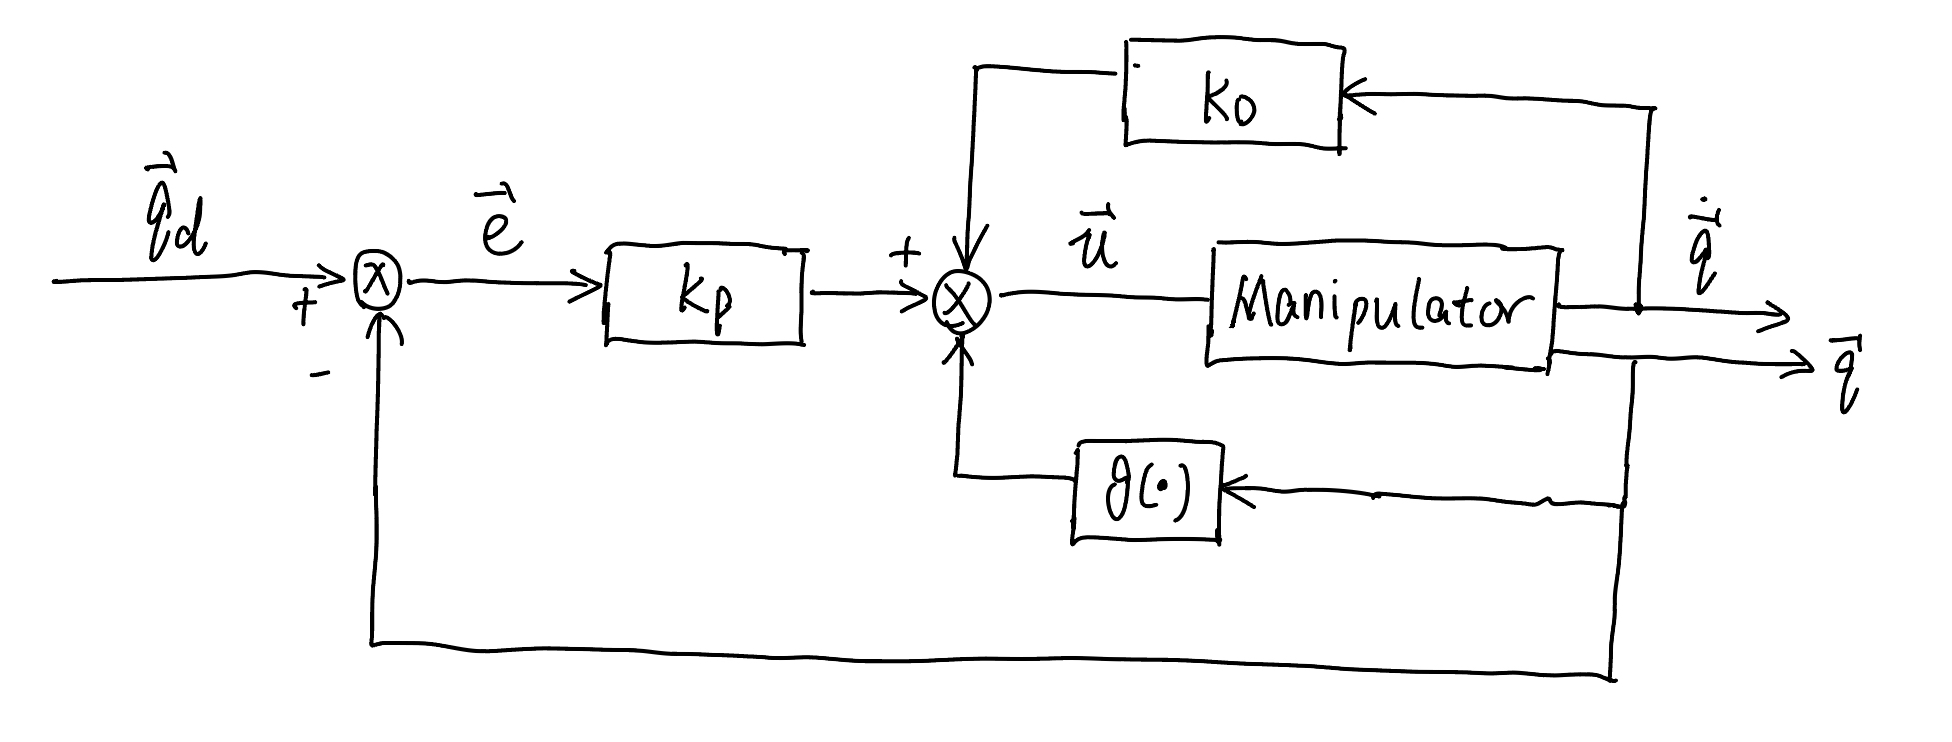
\includegraphics[max width=0.75\textwidth]{control/PD_control_with_gravity_compensation.jpeg}
    \caption{Control diagram of PD control with gravity compensation}
    \label{fig:enter-label}
\end{figure}





With the above controller (\ref{equ.controller2}), the time derivative of the Lyapunov function in (\ref{equ.lypuanovdot}) becomes
\begin{equation}
    \dot{V}=-\boldsymbol{\dot{q}}^T\boldsymbol{K}_D\boldsymbol{\dot{q}} \quad <0 \quad \forall \dot{\boldsymbol{q}}  \neq \mathbf{0}
\end{equation}
and thus, $V$ decreases long as $\dot{\boldsymbol{q}} \neq \mathbf{0}$ for all system trajectories. Thus, the controller manipulator will reach an equilibrium configuration, with condition $\dot{V}= 0$ and $\dot{\boldsymbol{q}}=\mathbf{0}$. To find the equilibrium configuration, we look at the manipulator dynamics under control

$$
\boldsymbol{B}(\boldsymbol{q}) \ddot{\boldsymbol{q}}+\boldsymbol{C}(\boldsymbol{q}, \dot{\boldsymbol{q}}) \dot{\boldsymbol{q}}+\boldsymbol{g}(\boldsymbol{q})=\boldsymbol{g}(\boldsymbol{q})+\boldsymbol{K}_{P} {\boldsymbol{e}}-\boldsymbol{K}_{D} \dot{\boldsymbol{q}}
$$

With the condition  $\dot{\boldsymbol{q}}=\mathbf{0}$, it follows that   $\ddot{\boldsymbol{q}} =\mathbf{0}$, and then from the above dynamics, we have
$$
\boldsymbol{K}_{P} {\boldsymbol{e}}=\mathbf{0} \quad\rightarrow\quad {\boldsymbol{e}}=\boldsymbol{q}_{d}-\boldsymbol{q} = \mathbf{0}
$$

Therefore, the manipulator will eventually reach equilibrium, which is exactly the desired configuration  $\boldsymbol{q}_{d}$.


The above derivation rigorously shows that any manipulator equilibrium posture is globally asymptotically stable under a controller with a PD linear action and a nonlinear gravity compensating action. Stability is ensured for any choice of $\boldsymbol{K}_{P}$ and $\boldsymbol{K}_{D}$, as long as these are positive definite matrices. 
The control law requires the on-line computation of the term $\boldsymbol{g}(\boldsymbol{q})$. 



\section{Controller II: Inverse Dynamics Control}
One limitation of the above controller is that the above controller can only follow a stationary desired $\boldsymbol{q}_d$, but is not good at tracking a changing desired joint signal: i.e., 

\begin{equation}
\label{equ.joint_signal}
\boldsymbol{q}_d(t),\quad\text{with} \quad \boldsymbol{\dot{q}}_d(t)\neq\boldsymbol{0} \quad \text{and} \quad \boldsymbol{\ddot{q}}_d(t)\neq\boldsymbol{0} 
\end{equation}

The approach of inverse dynamics control is trying to address the above limitation. The idea of  inverse dynamics control is to find a controller (\ref{equ.controller}) that can directly lead to  linearization of system dynamics. To do so, we set the controller (\ref{equ.controller}) in the following particular form:
\begin{shaded}
    \begin{equation}\label{equ:u}
    \boldsymbol{u}=\boldsymbol{B}(\boldsymbol{q}) \boldsymbol{y}+\boldsymbol{C}(\boldsymbol{q}, \dot{\boldsymbol{q}}) \dot{\boldsymbol{q}}+\boldsymbol{g}(\boldsymbol{q})
\end{equation}
\end{shaded}
where $\boldsymbol{y}$ is a new input vector whose expression is to be determined yet. The above controller directly leads to the controlled manipulator (\ref{equ.manipulator_control}) as
$$
 \boldsymbol{B}(\boldsymbol{q}) \ddot{\boldsymbol{q}}+\boldsymbol{C}(\boldsymbol{q}, \dot{\boldsymbol{q}}) \dot{\boldsymbol{q}}+\boldsymbol{g}(\boldsymbol{q})=\boldsymbol{B}(\boldsymbol{q}) \boldsymbol{y}+\boldsymbol{C}(\boldsymbol{q}, \dot{\boldsymbol{q}}) \dot{\boldsymbol{q}}+\boldsymbol{g}(\boldsymbol{q})
 $$
leading to 
\begin{equation}\label{equ.dyn_new}
\boldsymbol{\ddot{q}}=\boldsymbol{y} 
\end{equation}
Again, we will discuss how to set this new control input vector $\boldsymbol{y}$, but the particular form of controller (\ref{equ:u}) leads to a linear relationship between the input signal $\boldsymbol{y}$ and the manipulator's joint acceleration $\ddot{\boldsymbol{q}}$. 



The control diagram corresponding to the controller (\ref{equ:u}) is shown in Fig. \ref{fig:2}. The controller (\ref{equ:u}) is termed inverse dynamics control as it is based on the computation of  inverse dynamics. From (\ref{equ.dyn_new}, the controlled manipulator system   is linear and decoupled with respect to new input $\boldsymbol{y}$.

\begin{figure}[H]
    \centering
    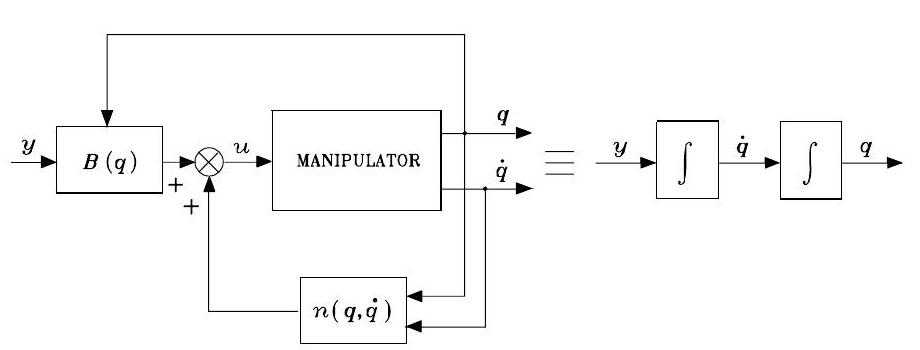
\includegraphics[max width=0.55\textwidth]{control/inverse dynamics control.jpeg}
    \caption{Exact linearization performed by inverse dynamics control}
    \label{fig:2}
\end{figure}




Thus, the manipulator control problem is reduced to that of finding a  control input signal $\boldsymbol{y}$. To this end, 
\begin{shaded}
    \begin{equation}\label{equ.y}
    \boldsymbol{y}=\ddot{\boldsymbol{{q}}}_d+\boldsymbol{K}_{P} ({\boldsymbol{q}}_{d}-\boldsymbol{q})+\boldsymbol{K}_{D} (\dot{\boldsymbol{q}}_{d}-\dot{\boldsymbol{q}})
\end{equation}
\end{shaded}

Here,  $\boldsymbol{K}_{P}$ and $\boldsymbol{K}_{D}$ are positive definite matrices.
Plugging the above $\boldsymbol{y}$ signal into (\ref{equ.dyn_new}) leads to
\begin{equation}\label{equ.error_dyn}
    (\ddot{\boldsymbol{{q}}}_d-\ddot{\boldsymbol{q}})+\boldsymbol{K}_{P} ({\boldsymbol{q}}_{d}-\boldsymbol{q})+\boldsymbol{K}_{D} (\dot{\boldsymbol{q}}_{d}-\dot{\boldsymbol{q}})=\boldsymbol{0}
\end{equation}

Again, if we define the error $\boldsymbol{e}={\boldsymbol{q}}_{d}-{\boldsymbol{q}}$, the above (\ref{equ.error_dyn}) becomes the following error dynamics
\begin{equation}\label{equ.error_dyn}
    \ddot{\boldsymbol{e}}+\boldsymbol{K}_{P} \dot{\boldsymbol{e}}+\boldsymbol{K}_{D} {\boldsymbol{e}}=\boldsymbol{0}
\end{equation}
expressing the dynamics of position error  while tracking the given trajectory. This is a standard second-order error system, where its convergence depends on the value of $\boldsymbol{K}_P$ and $\boldsymbol{K}_D$. 
Particularly, we usually choose 
\begin{equation}\label{equ.kpkd}
    \boldsymbol{K}_{P}=\operatorname{diag}\left\{\omega_{n 1}^{2}, \ldots, \omega_{n n}^{2}\right\} \quad \boldsymbol{K}_{D}=\operatorname{diag}\left\{2 \zeta_{1} \omega_{n 1}, \ldots, 2 \zeta_{n} \omega_{n n}\right\}
\end{equation}
Then, the controlled manipulator dynamics is replaced with $n$ linear and decoupled second-order subsystems. For each joint $i$, please see my control background notes for how the values of the damping ratio $\zeta_i$ and natural frequency $\omega_{ni}$ can affect the trajectory of $\boldsymbol{e}(t)$. 








The resulting block scheme is illustrated in Fig. \ref{fig:3}. Notice that the inverse dynamics controller requires computation of the inertia matrix $\boldsymbol{B}(\boldsymbol{q})$, $\boldsymbol{C}(\boldsymbol{q}, \dot{\boldsymbol{q}})$, and $\boldsymbol{g}(\boldsymbol{q})$.  
 Nonetheless, this technique is based on the assumption of perfect cancellation of dynamic terms, and then it is quite natural to raise questions about sensitivity and robustness problems due to unavoidably imperfect compensation.




\begin{figure}[H]
    \centering
    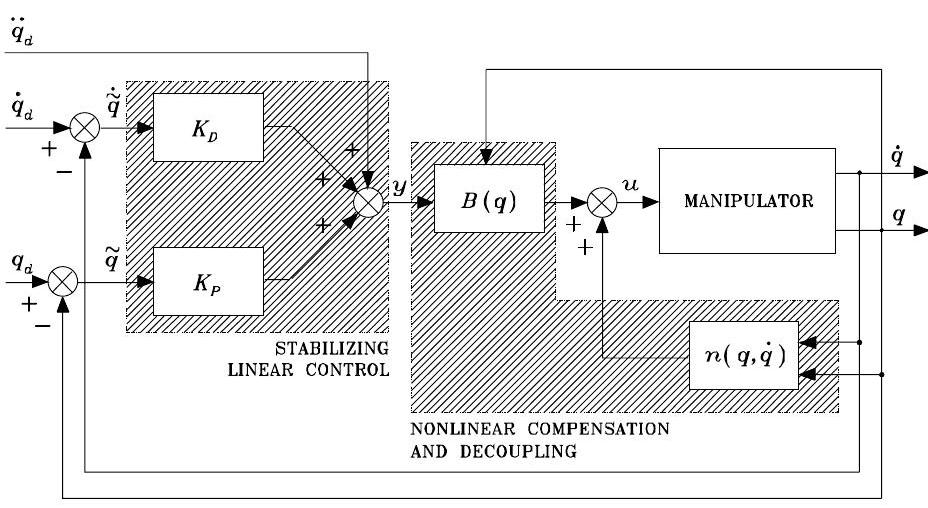
\includegraphics[max width=0.75\textwidth]{control/inverse dynamics control2.jpeg}
    \caption{Control diagram of joint space inverse dynamics control}
    \label{fig:3}
\end{figure}





\end{document}